\chapter{TD strain tensor with surface relaxation}
\label{Chap:strainMatrix}

The strain tensor of a semi-infinite threading dislocation normal to a surface, $\epsilon_{ij}$,  is shown below as contour plots for each strain tensor component. I'm showing these images in the strain tensor matrix form:
\begin{equation*}
    \epsilon_{ij} = \begin{pmatrix}
    \epsilon_{11} & \epsilon_{12} & \epsilon_{13} \\
    \epsilon_{21} & \epsilon_{22} & \epsilon_{23} \\
    \epsilon_{31} & \epsilon_{32} & \epsilon_{33} \\
    \end{pmatrix}.
\end{equation*}

Where the dislocation line is along z or index 3 in this notation. The elastic strain has the following property : $\epsilon_{ij}=\epsilon_{ji}$ making these matrices symmetric with respect to their diagonal, which is why there are only maximum 6 plots per image, \ie diagonal terms plus 3. Fig.~\ref{Fig:screwMatrix} shows the top view of strain components as contour plots for a screw threading dislocation and   Fig.~\ref{Fig:edgeMatrix} for an edge TD. 

The colour map for all the plots in a matrix has the same limits for comparison. The $\epsilon_31$ and $\epsilon_32$ are the biggest components for the screw TD (Fig.~\ref{Fig:screwMatrix}). This is perhaps not very easy to see because I choose I narrow colour range in order to pull out some features in the other images but it did mean, unfortunately that the peak in values in $\epsilon_31$ and $\epsilon_32$ is outside the colour range and shown here as white. Another way to read this matrix is to say that most of the strain of the screw threading dislocation in a semi-infinite medium is the shear strain normal to the plane xy. Nothing new so far. 

Similarly, for the edge TD, shown in an identical manner in Fig.~\ref{Fig:edgeMatrix}, where I choose better colour map limits, the main components are $\epsilon_11$, $\epsilon_12$, $\epsilon_22$, \ie all the strain contained entirely in the plane xy. 
%---------
\begin{sidewaysfigure}[ht]
    \centering
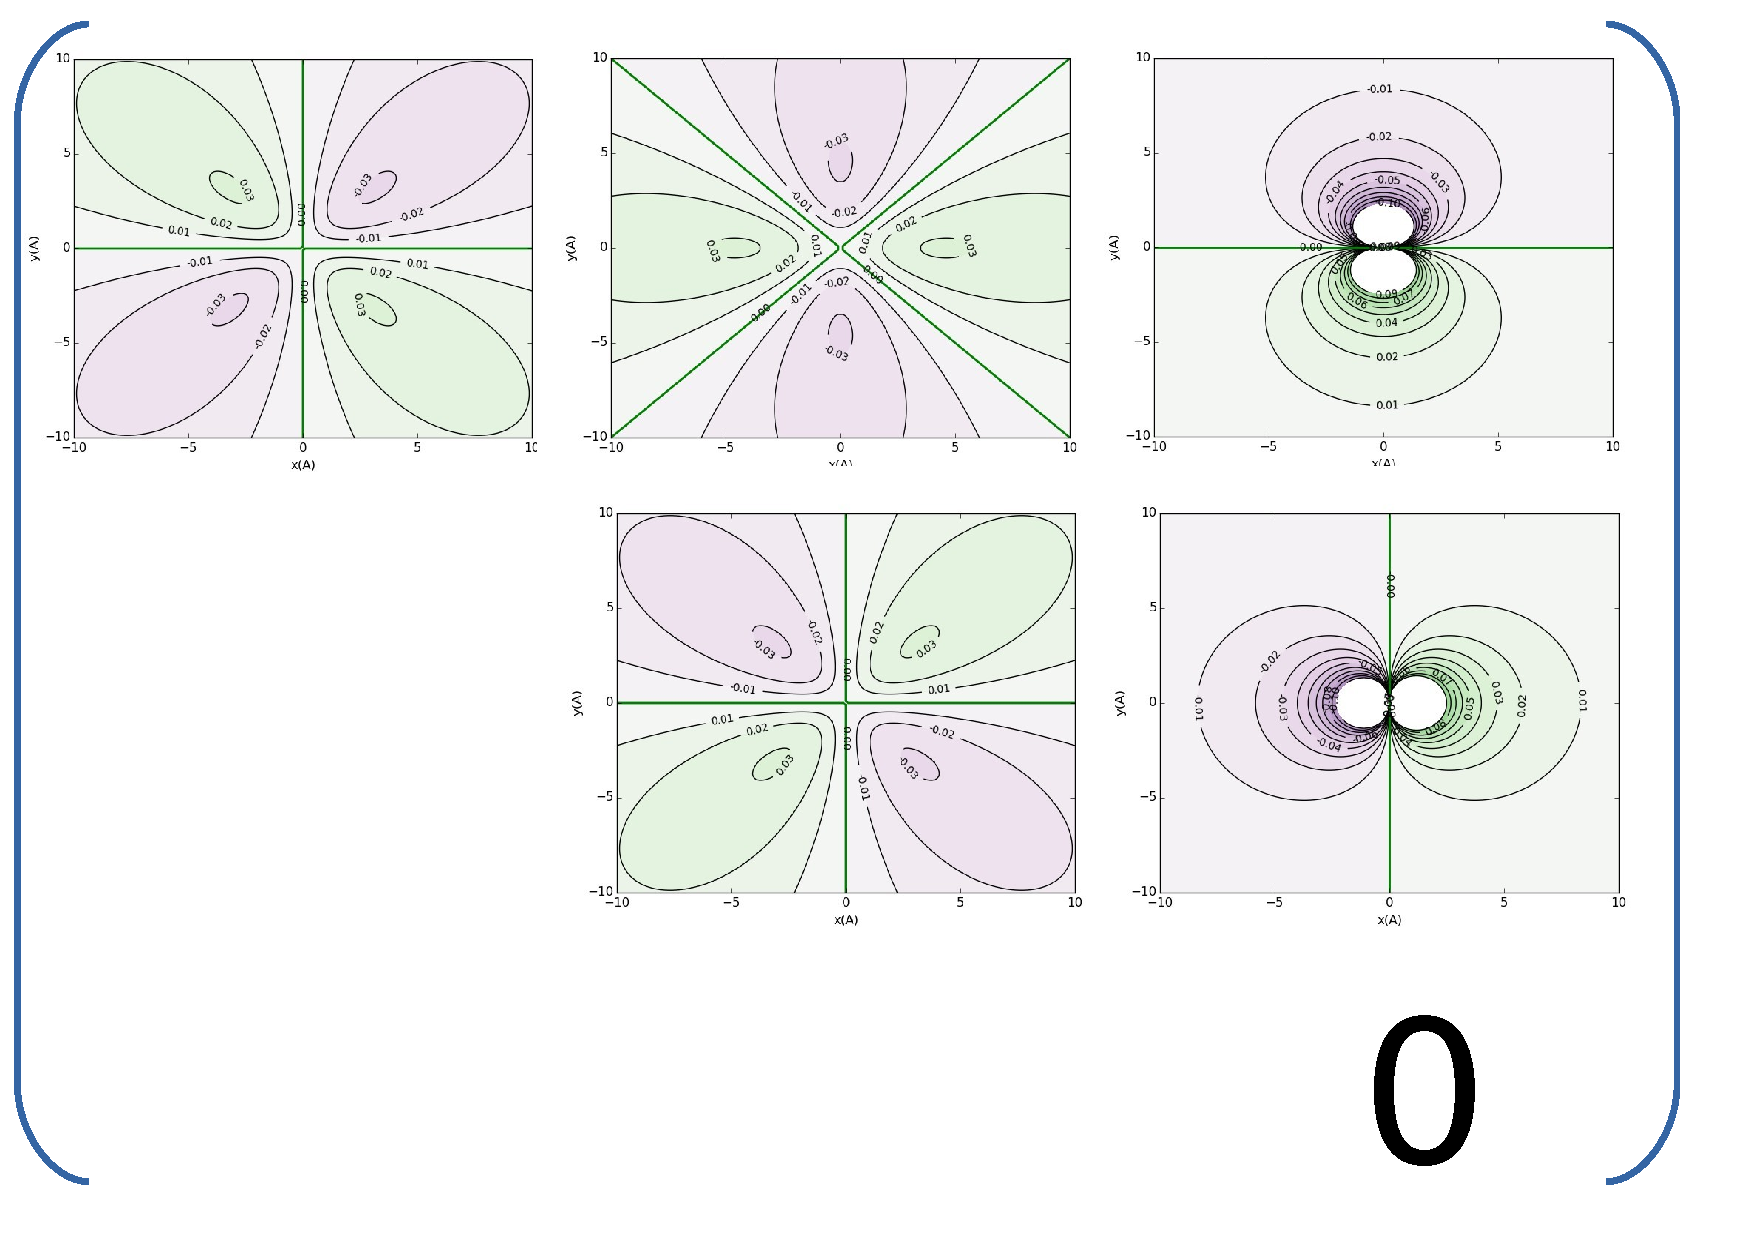
\includegraphics[width=1\linewidth]{Figures/screw_matrix.pdf}
\caption[Screw TD strain tensor.]{Strain field tensor components of a screw TD in GaN normal to a surface as contour plots. The strain is plotted on a $10 \times 10$ \si{\angstrom} plane centred on the dislocation and \SI{2}{\angstrom} below the surface.  }
\label{Fig:screwMatrix}
\end{sidewaysfigure}
%---------



%---------
\begin{sidewaysfigure}[ht]
    \centering
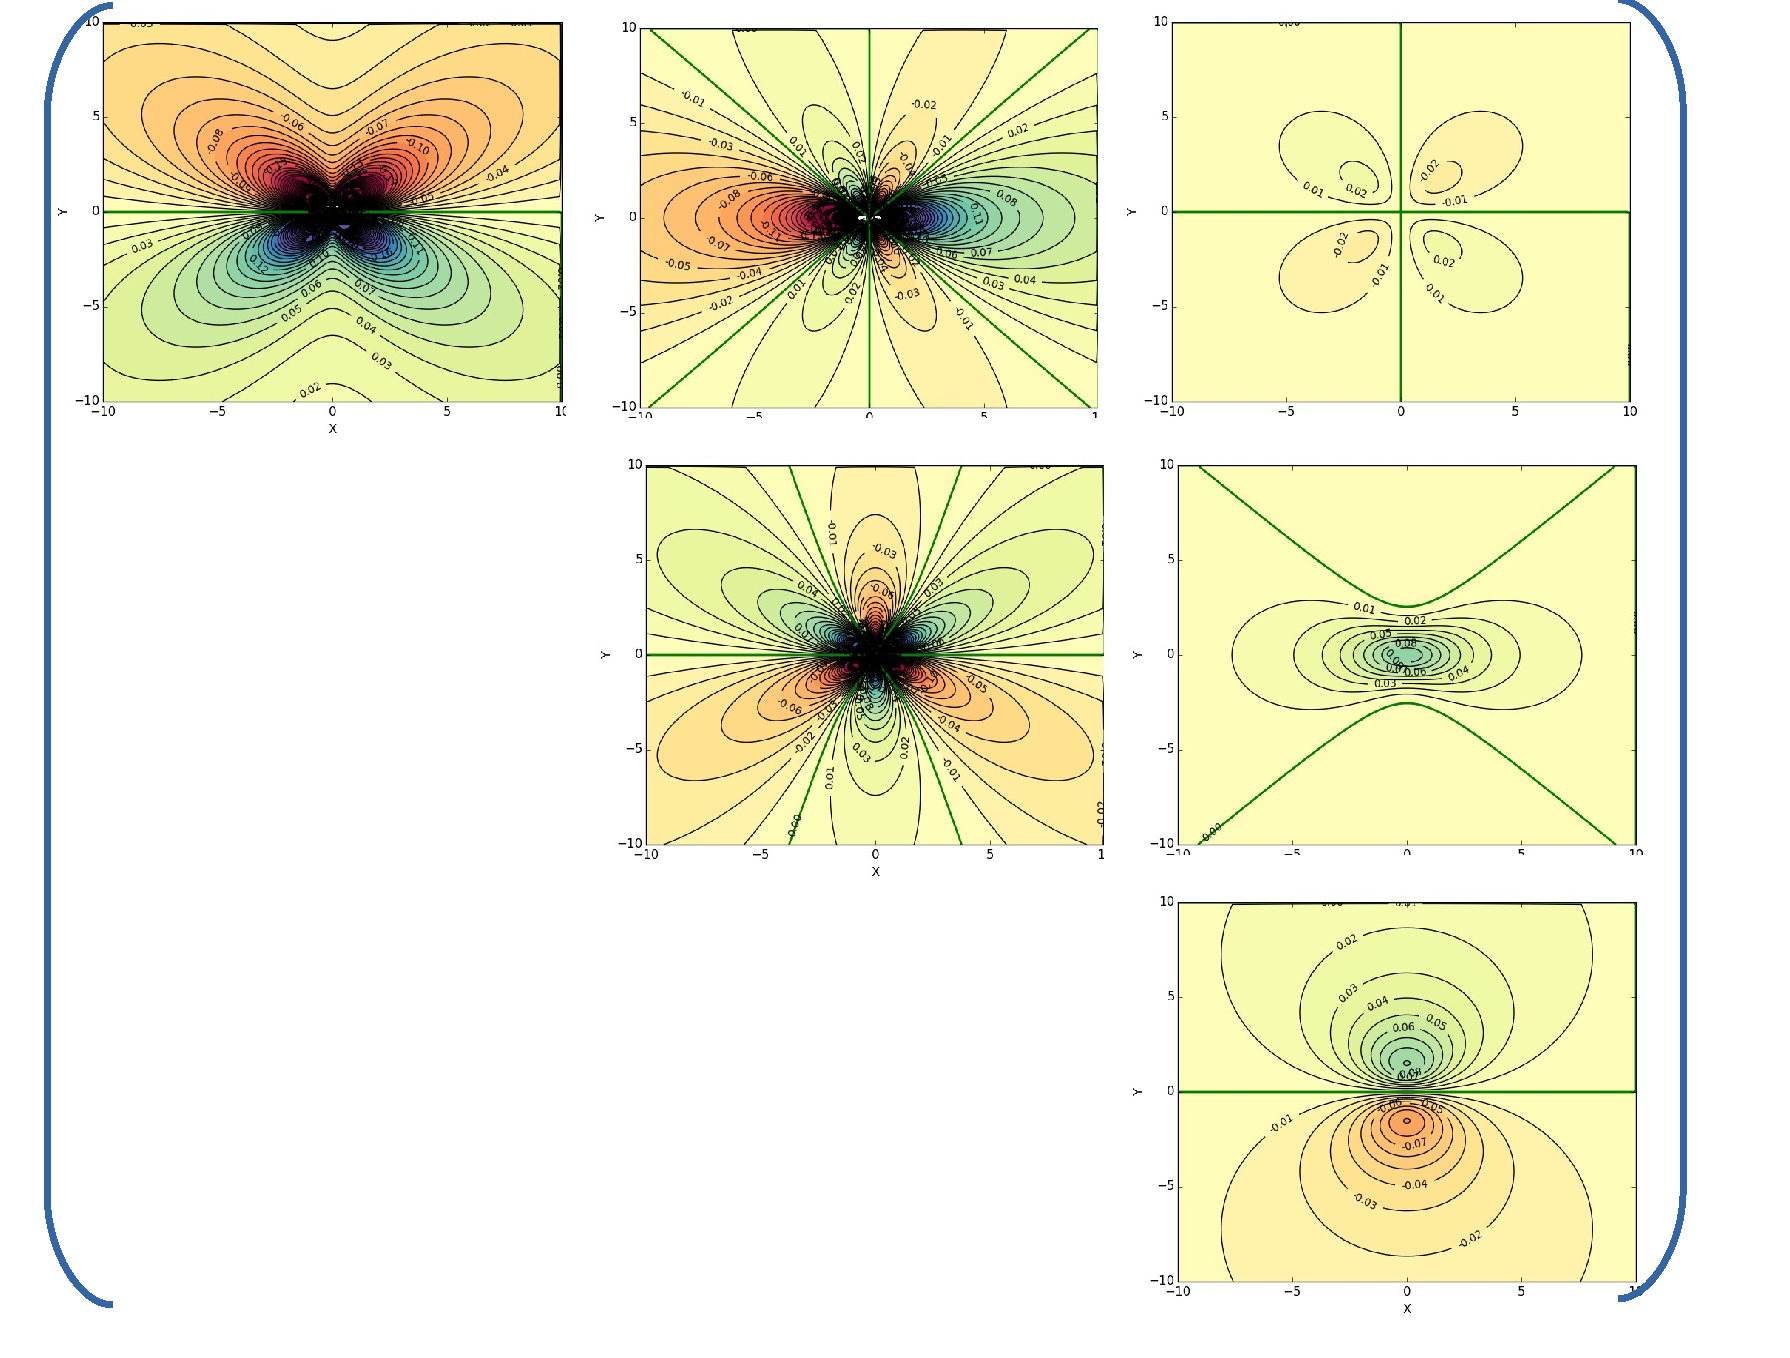
\includegraphics[width=1\linewidth]{Figures/edge_matrix.pdf}
\caption[Edge TD strain tensor.]{Strain field tensor components of an edge TD in GaN normal to a surface as contour plots. The strain is plotted on a $10 \times 10$ \si{\angstrom} plane centred on the dislocation and \SI{2}{\angstrom} below the surface.  }
\label{Fig:edgeMatrix}
\end{sidewaysfigure}
%---------

